%12/7/2023 need to do a full rec and comparison with Waganer to hand, also to include IAEA to hand... another iteration needed

\subsection{Cost Category 21: Structures and Improvements}

This account covers all direct costs associated with the construction and provision of physical plant buildings and structures. Key elements include the reactor, turbine, electrical equipment, and cooling system structures, along with site improvements, facilities, and miscellaneous building work. The costs for these structures, especially the heat island and turbine buildings, represent a significant portion of the total cost of the facility. For instance, the Heat Island Building is noted for its compact design, thick radiation shielding walls, and inclusion of access corridors and hot cell, leading to its estimated cost. The Turbine Building, housing turbines and auxiliary equipment, is also a major cost component, with its size and cost dependent on the size of turbines and equipment. Additional facilities like the Hot Cell, Service Water, and Fuel Handling Buildings, Control Room, On-Site AC Power, and other administrative and service buildings are also included, each having distinct scaling factors and cost estimates based on their specific functions and requirements within the power plant. We provide a detailed cost estimation approach for each of these buildings, reflecting their critical role in the overall construction and operation of the energy plant.\\

\begin{figure}[h!] 
\centering 
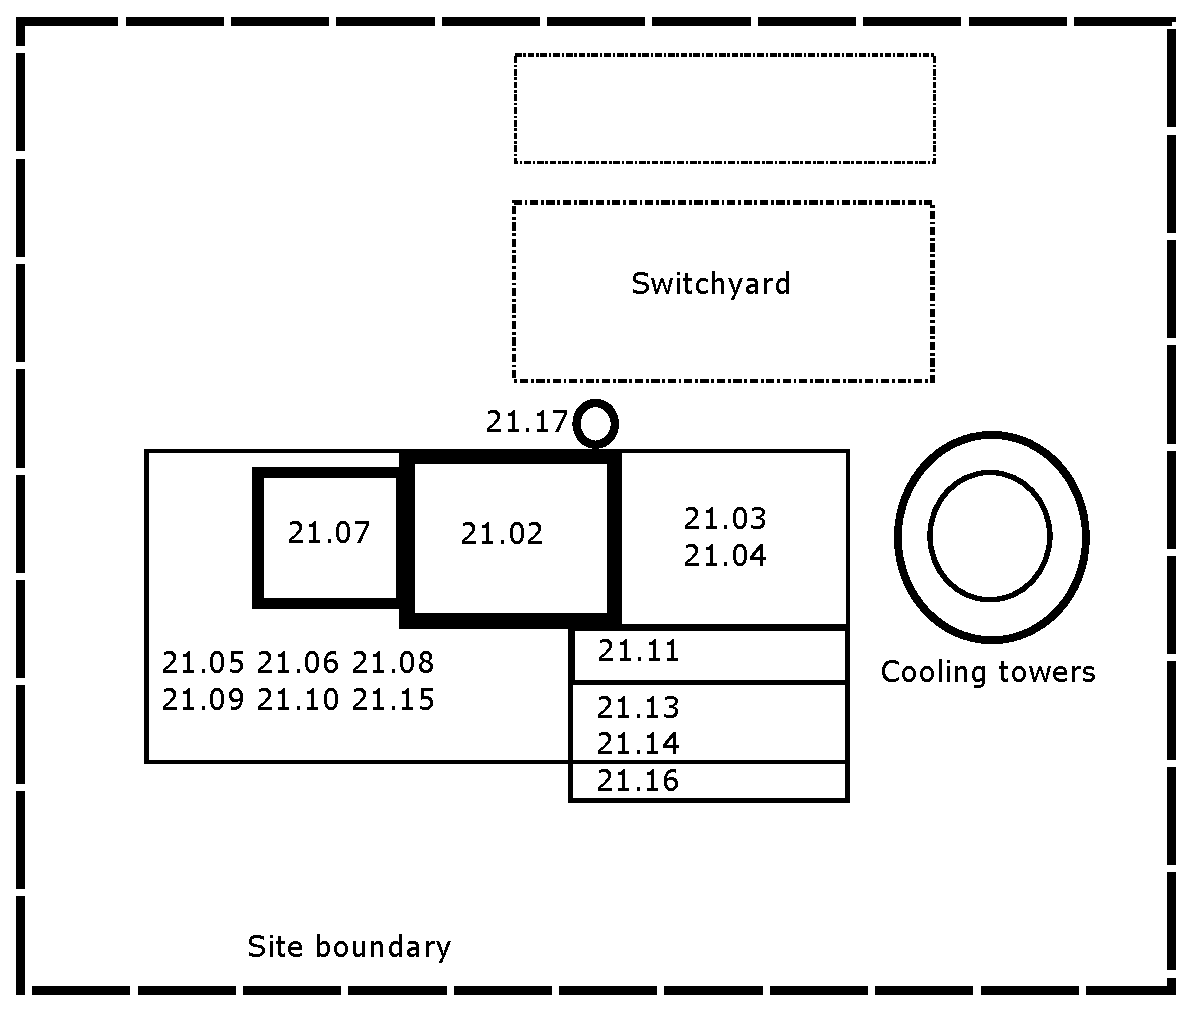
\includegraphics[scale=0.6]{StandardFigures/siteplan2023.eps} 
\caption{Site plan with labels according to the cost accounts described in the text.  Cooling towers and Switchyards are costed elsewhere.} 
\label{fig:site} 
\end{figure} 



 \textbf{2020 Update} 
\emph{Scope: } 
Site preparation and yard work, reactor building, turbine building, security building and gatehouse, control and administrative buildings, maintenance shop, any other site structures and facilities. 
 \emph{Previous values:} CAD calculations for building volumes and concrete volumes multiplied by materials costs. 
Min \$373/kW, Average \$606/kW, Max \$1,142/kW. 
\emph{Reduction strategies: } 
Minimal reactor building size and wall/ceiling thickness (while fully preserving safety); minimal volumes for concrete and other materials (expensive concrete vs. inexpensive soil or sand, perhaps as inner fill material within metal or concrete walls); avoidance of unnecessary buildings in plant design; reuse of buildings if an existing power plant site; modular construction, as in Wartsila Modular Block. 
\emph{Updated value: } 
Average of previous value reduced by 25 \% with implementation of feasible strategies listed above. \$606/kW $\times$ - 0.25 = \$470/kW, giving a total for CAS21 of C210000 M \$. 
%\emph{2023 Updated value: } 
%Buildings now built using a bottoms up approach, totaling 450.0 M \$.    
%\begin{figure}[h!] 
%\centering 
%\includegraphics[width =1\linewidth]{/home/ahigginbottom/Desktop/CODE050202023/CATF_DT/MIf_site(1).pdf} 
%\caption{Site, buildings built from the ground up and costed individually.} 
%\label{fig:site} 
%\end{figure} 

\begin{table}[h!] 
    \begin{tiny}
    \centering
    \begin{tabular}{l l  c c c c c c c c c }
Cost Category	&	Building	&	Wall materials	&	 \$/kW gross	&	L	&	W	&	H	&	Vol	&	Esc year	&	Esc	&\$/kW gross	\\
21.01.00	&	Site improve. \& facs	&		&	20.7	&		&		&		&		&	2019	&	1.19	&	24.6	\\
21.02.00	&	Heat Island Building	&	Concrete \& Steel	&	131.6	&	48.3	&	48.3	&	60	&	140000	&	2009	&	1.42	&	186.8	\\
21.03.00	&	Turbine building	&	Steel 	&	45.3	&	48.3	&	48.3	&	30	&	70000	&	2019	&	1.19	&	54.0	\\
21.04.00	&	Heat rejection 	&	Concrete \& Steel	&	31.7	&	48.3	&	48.3	&	15	&	35000	&	2019	&	1.19	&	37.8	\\
21.05.00	&	Power supplies	&	Concrete \& Steel	&	9.1	&	9.7	&	9.7	&	6.0	&	560	&	2019	&	1.19	&	10.8	\\
21.06.00	&	Plant aux.	&	Concrete \& Steel	&	4.5	&	4.8	&	4.8	&	3.0	&	70	&	2019	&	1.19	&	5.4	\\
21.07.00	&	Hot cell	&	Concrete \& Steel	&	65.8	&	24.2	&	24.2	&	60	&	35000	&	2013	&	1.42	&	93.4	\\
21.08.00	&	Heat Island Services	&	Steel frame	&	13.2	&	4.8	&	4.8	&	10	&	233	&	2013	&	1.42	&	18.7	\\
21.09.00	&	Service water	&	Steel frame	&	0.2	&	1.3	&	4.0	&	4.0	&	21	&	2019	&	1.19	&	0.3	\\
21.10.00	&	Fuel storage	&	Steel frame	&	0.9	&	5.0	&	15.0	&	2.5	&	188	&	2019	&	1.19	&	1.1	\\
21.11.00	&	Control room	&	Steel frame	&	0.7	&	4.0	&	12.0	&	2	&	96	&	2019	&	1.19	&	0.9	\\
21.12.00	&	Onsite AC power	&	Steel frame	&	0.7	&	3.6	&	10.8	&	1.8	&	70	&	2019	&	1.19	&	0.8	\\
21.13.00	&	Administration	&	Steel frame	&	3.7	&	20.0	&	60.0	&	10	&	12000	&	2019	&	1.19	&	4.4	\\
21.14.00	&	Site services	&	Steel frame	&	1.3	&	7.3	&	22.0	&	3.7	&	593	&	2019	&	1.19	&	1.6	\\
21.15.00	&	Cryogenics	&	Steel frame	&	2.0	&	11.0	&	33.0	&	5.5	&	2003	&	2019	&	1.19	&	2.4	\\
21.16.00	&	Security	&	Steel frame	&	0.7	&	4.0	&	12.0	&	2	&	96	&	2019	&	1.19	&	0.9	\\
21.17.00	&	Ventilation stack	&	Steel \& concrete 	&	22.7	&		&		&	120	&		&	2019	&	1.19	&	27.0	\\
21.98.00	&	Spare parts allowance	&		&		&		&		&		&		&		&		&	0.0	\\
21.99.00	&	Contingency allowance	&		&	0.0	&		&		&		&		&		&		&	0.0	\\
21.00.00	&	Structures and site facs	&		&	354.9	&		&		&		&		&		&		&	470.7	\\
    \end{tabular}															
    \end{tiny} 																	
    \caption{Cost categories for buildings, and their cost estimation}	
    \label{tab:buildings}
\end{table} 











\subsection*{Cost Category 21.1 Site Preparation/Yard Work}
Includes clearing, grubbing, scraping, geo-technical work, site cut, fill and compact, drainage, fences, landscaping, etc.  Cost is \$ C210100 M using NETL Reference case B12A, account 13, bare erected costs for 13.1 site preparation and 13.2 site improvements, for a 686MW gross power plant in 2019 \$, applying escalation per table \ref{tab:buildings}.

\subsection*{Cost Category 21.2 Heat Island Building}
Includes installation, labor, and materials for concrete and metalwork for the building surrounding and supporting the heat island, including the containment structure. Also includes the biological shielding, structural excavation and backfill, foundations, walls, slabs, siding, roof, architectural finishes, elevators, lighting, HVAC (general building service), fire protection, plumbing, and drainage. Cost is \$ C210200 M using Waganer cost reference for ARIES-ST.


\subsection*{Cost Category 21.3 Turbine Generator Building}
Includes installation, labor, and materials for concrete and structural metalwork for the building surrounding and supporting the turbine generator(s). (For concepts that do not produce electricity, this account can be replaced with appropriate energy product buildings.) Also includes structural excavation and backfill, foundations, walls, slabs, siding, roof, architectural finishes, elevators, lighting, HVAC, fire protection, plumbing, and drainage.  This building contains the turbines and heat exchangers. Cost is \$ C210300 M using NETL Reference case B12A, account 14.3, turbine building bare erected costs for a 686MW gross power plant in 2019 \$, apply escalation per table \ref{tab:buildings}.

\paragraph{}
The rest of the 21 series accounts are for other support buildings on the site. Modular concepts might have a separate building to house centralized functions for all modules, such as an external control room. Here, the building costs are for the complete civil structure, including structural excavation and backfill, foundations, finishes, and building services such as elevators, lighting, HVAC, fire protection, or domestic water and drainage, but do not include the specialized equipment within.

\begin{itemize}
\item Cost Category 21.04 - Heat Rejection Building. This account covers the costs associated with the systems needed for rejecting heat from the power plant, scaled to the rejected thermal power. Cost is \$ C210400 M using NETL Reference case B12A, account 14.2, boiler building bare erected costs for a 686MW gross power plant in 2019 \$, apply escalation per table \ref{tab:buildings}. 
\item Cost Category 21.05 - Electrical Equipment \& Power Systems Building. It includes the costs for all electrical equipment and power systems, scaling with the net electrical power output of the plant. Cost is \$ C210500 M, using a smaller version of the turbine building - multiple floors, concrete, per table \ref{tab:buildings}.
\item Cost Category 21.06 - Plant Auxiliary Systems Building. This account addresses the costs of auxiliary systems in the plant, such as compressed air, inert gas storage, and distribution systems, scaling with the gross electrical power. Cost is \$ C210600 M as smaller version of the turbine building - multiple floors, concrete, per table \ref{tab:buildings}. 
\item Cost Category 21.07 - Hot Cell Building. The cost for the Hot Cell Building, designed for handling large and hazardous components, is scaled in relation to the Reactor Building.  Cost is \$ C210700 M as a smaller version of the Heat Island Building by 50\%, per table \ref{tab:buildings}.  
\item Cost Category 21.08 - Heat Island Service Building. This includes the costs for a service building specific to the reactor, similar in cost to structures in projects. Cost is \$ C210800 M as smaller version of the Heat Island Building by 10\%, per table \ref{tab:buildings}.  
\item Cost Category 21.09 - Service Water Building. The Service Water Building, essential for the plant’s water supply needs, has its costs modeled after similar structures in other power plant projects. Cost is \$ C210900 M following NETL Reference case B12A, account 14.5, circulation water pumphouse and 14.6 water treatment building bare erected costs for a 686MW gross power plant in 2019 \$, applying escalation per table \ref{tab:buildings}.
\item Cost Category 21.10 - Fuel Handling and Storage Building. This account covers the costs for buildings related to handling and storing fuel, scaled according to tritium usage or fusion power. Cost is \$ C211000 M, scaled relative to the administration building per table \ref{tab:buildings}. 
\item Cost Category 21.11 - Control Room Building. It encompasses the expenses for the control room building, essential for plant operations, with costs similar to those in previous plant designs.  Cost is \$ C211100 M scaled relative to the administration building per table \ref{tab:buildings}. 
\item Cost Category 21.12 - On-Site AC Power Building. This account includes the costs for buildings housing on-site alternating current (AC) power systems, comparable to similar structures in other projects.  Cost is \$ C211200 M scaled relative to the administration building per table \ref{tab:buildings}. 
\item Cost Category 21.13 - Administrative Building. It covers the costs associated with the construction of the plant’s administrative building, with cost estimates based on previous similar projects. Cost is \$ C211300 M as NETL Reference case B12A, account 14.4, administration building building bare erected costs for a 686MW gross power plant in 2019 \$, apply escalation per table \ref{tab:buildings}. 
\item Cost Category 21.14 - Site Service Building. This account entails the costs for a building providing various site services, with costs aligned with those in comparable plant designs. Cost is \$ C211400 M as NETL Reference case B12A, account 14.7, machine shop building bare erected costs for a 686MW gross power plant in 2019 \$, apply escalation per table \ref{tab:buildings}. 
\item Cost Category 21.15 - Cryogenic and Inert Gas Storage Building. It includes the costs for buildings that store cryogenic and inert gases, essential for plant operations.  Cost is \$ C211500 M Like site services, per table \ref{tab:buildings}. 
\item Cost Category 21.16 - Security Building. The Security Building account covers the costs for structures dedicated to the plant’s security and surveillance. Cost is \$ C211600 M like administration, see table \ref{tab:buildings}. 
\item Cost Category 21.17 - Ventilation Stack. This account addresses the costs of the ventilation stack, a crucial component for plant ventilation and safety. Cost is \$ C211700 M as NETL Reference case B12A, account 7, ventilation stack bare erected costs for a 686MW gross power plant in 2019\$, apply escalation per table \ref{tab:buildings}.
\end{itemize}









